\begin{center}
\textbf{
\MakeUppercase{Приложение А}\\
(обязательное)\\
Исходный код}
\end{center}
\addcontentsline{toc}{section}{Приложение А. Исходный код}

\lstinputlisting{inc/src/rx-feedback-state.swift}

\newpage

\newcommand{\pra}{
\begin{center}
\textbf{
\MakeUppercase{Приложение Б}\\
(информационное)\\
Результаты проверки уникальности текста}
\end{center}
\addcontentsline{toc}{section}{Приложение Б. Результаты проверки уникальности текста}
}

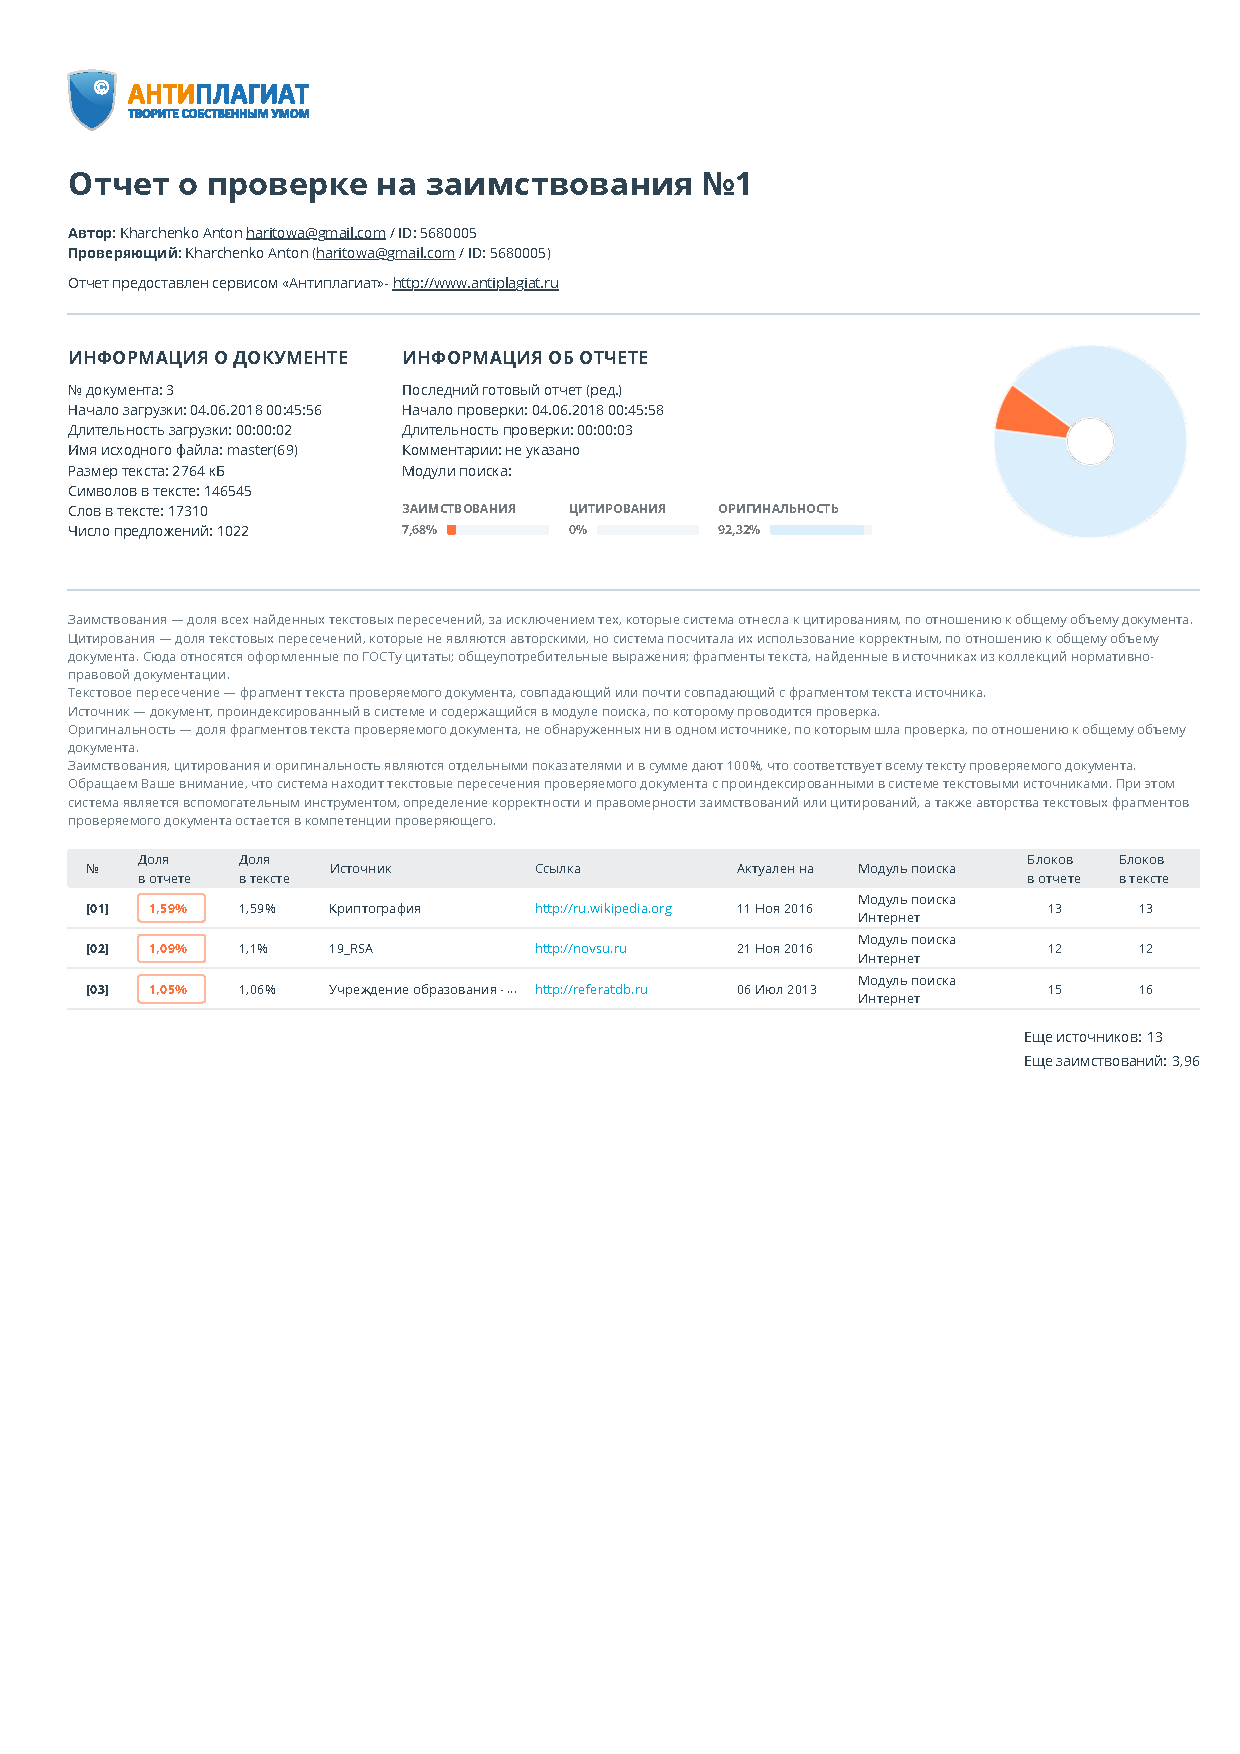
\includepdf[scale=0.8,pages=-,pagecommand={\pra}]{inc/pdf/antiplagiat.pdf}
\newpage


\begin{center}
\textbf{
\MakeUppercase{Приложение В}\\
(обязательное)\\
Ведомость}
\end{center}
\addcontentsline{toc}{section}{Приложение В. Ведомость}

\newpage
\pagestyle{empty}
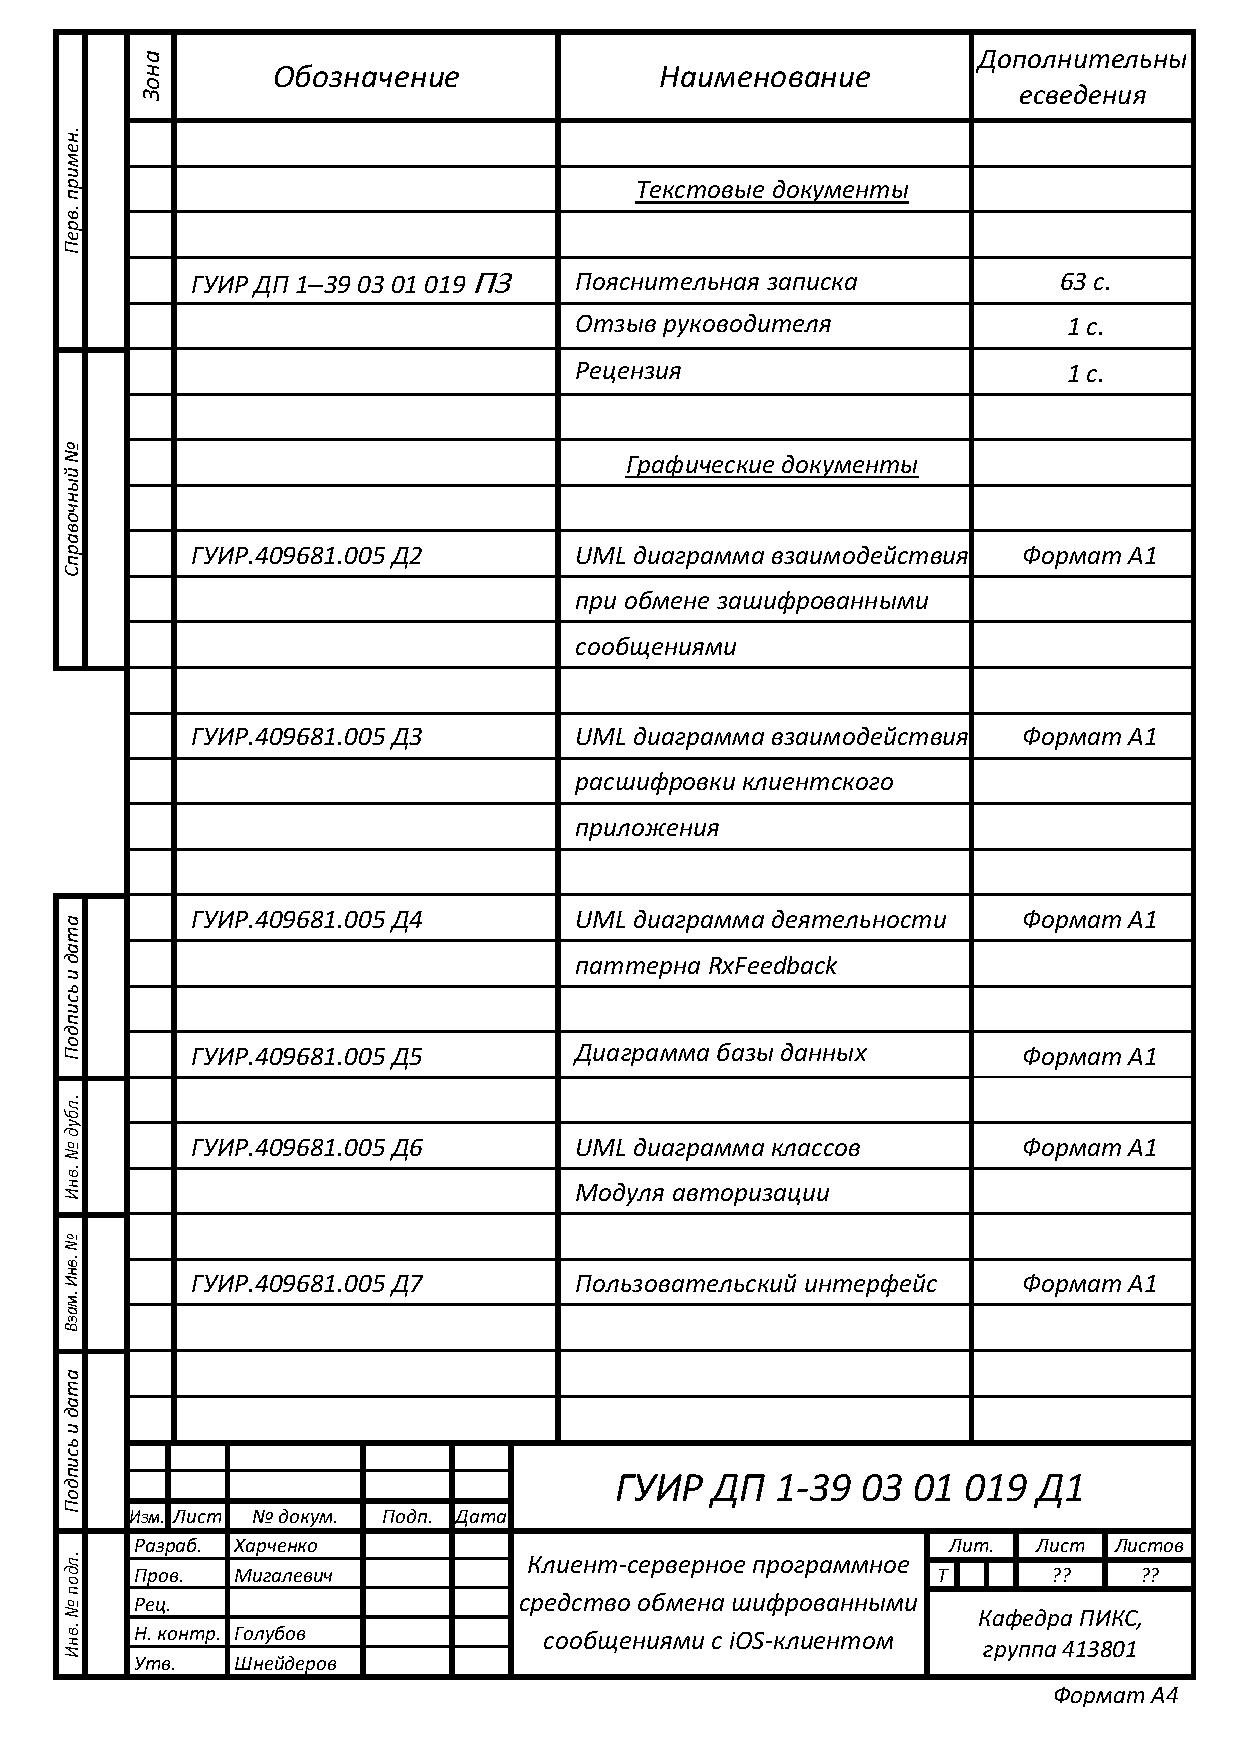
\includepdf[pages=-,pagecommand={}]{inc/pdf/vedomost.pdf}
\pagestyle{fancy}